\chapter{Application Layer}
\label{chapter:applicationlayer}

% OVERVIEW
\section{Overview}
This section gives an overview over the components of the application layer of ACE. Figure \ref{applicationlayer_ace_overview} shows the graphical user interface (GUI) with all components. Each component is explained in detail in section \ref{applicationlayer_component_desc}.
\begin{figure}[H]
\begin{center}
  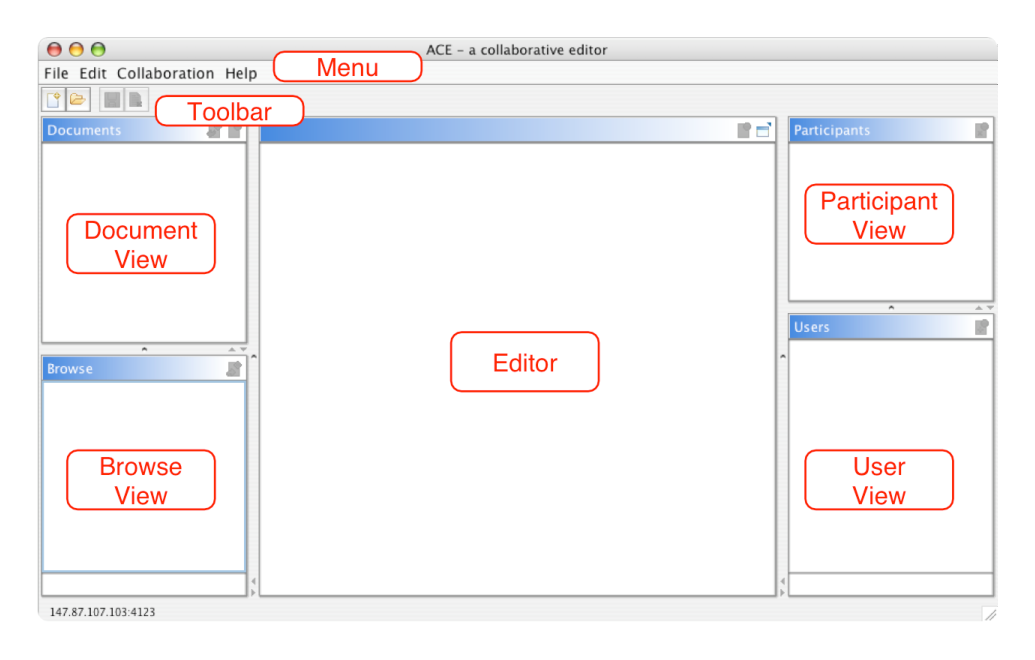
\includegraphics[height=3.135in, width=5.01in]{../images/finalreport/application_ace_overview.eps}
\caption{ACE Overview}
\label{applicationlayer_ace_overview}
\end{center}
\end{figure}
On the top of the window are the \emph{Menu Bar} and the \emph{Tool Bar}. The \emph{Menu Bar} is split into four menus which contain actions associated to the categories \emph{File}, \emph{Edit}, \emph{Collaboration} and \emph{Help}. Below the \emph{Menu Bar} is the \emph{Tool Bar} that contains the most commonly used actions.

Below the \emph{Tool Bar} are the four views and the editor component. The \emph{Document View} shows the currently open documents, the \emph{Browse View} contains all documents that have been discovered (shared by other users), the \emph{User View} shows all users running ACE and the \emph{Participant View} displays a list of users currently editing the selected document.

The \emph{Status Bar} can be found at the bottom of the application. It is a label diplaying the local IP address.

% COMPONENTS
\section{Components}
\label{applicationlayer_component_desc}

% FRAME
\subsection{Frame}
\label{applicationlayer_frame_desc}
The \emph{Main Frame} of the application layer is a \texttt{Persistent\-Frame} (not yet fully implemented). A \texttt{Persistent\-Frame} is a \texttt{JFrame} that saves the last position and size of it. Each time the application is started, the frame has the same position as the last time the application has been terminated. It is possible to add GUI components like a \texttt{JMenu\-Bar}, a \texttt{JTool\-Bar}, a \emph{Status Bar} and the content pane (\texttt{JPanel}). Further, the \texttt{Persistent\-Frame} has a \texttt{Window\-Listener} to catch the window closing event and forward it to the \texttt{Exit\-Action}.

% MENU
\subsection{Menu}
The menu bar is created by the method \texttt{createMenuBar()} of the \texttt{Application\-Factory} (see section \ref{applicationlayer_applicationfactory}).

% TOOLBAR
\subsection{Toolbar}
Toolbars are used to make the most commonly used actions easily accessible. The application layer uses a \texttt{JTool\-Bar} for that purpose. It is created by the \texttt{Application\-Factory} in the method \texttt{create\-Tool\-Bar()}.

% VIEWS
\subsection{Views \& View Controllers}
This section gives an overview of all the used \texttt{View} classes and how they are managed by their associated \texttt{View\-Controlle} classes. Figure \ref{application_views_controllers} shows the class diagram of the \texttt{Views} and \texttt{ViewControllers}. NOTE: the abbreviation \emph{ISC} stands for \texttt{Item\-Selection\-Change}.

\subsubsection{Overview}
\begin{figure}[H]
\begin{center}
  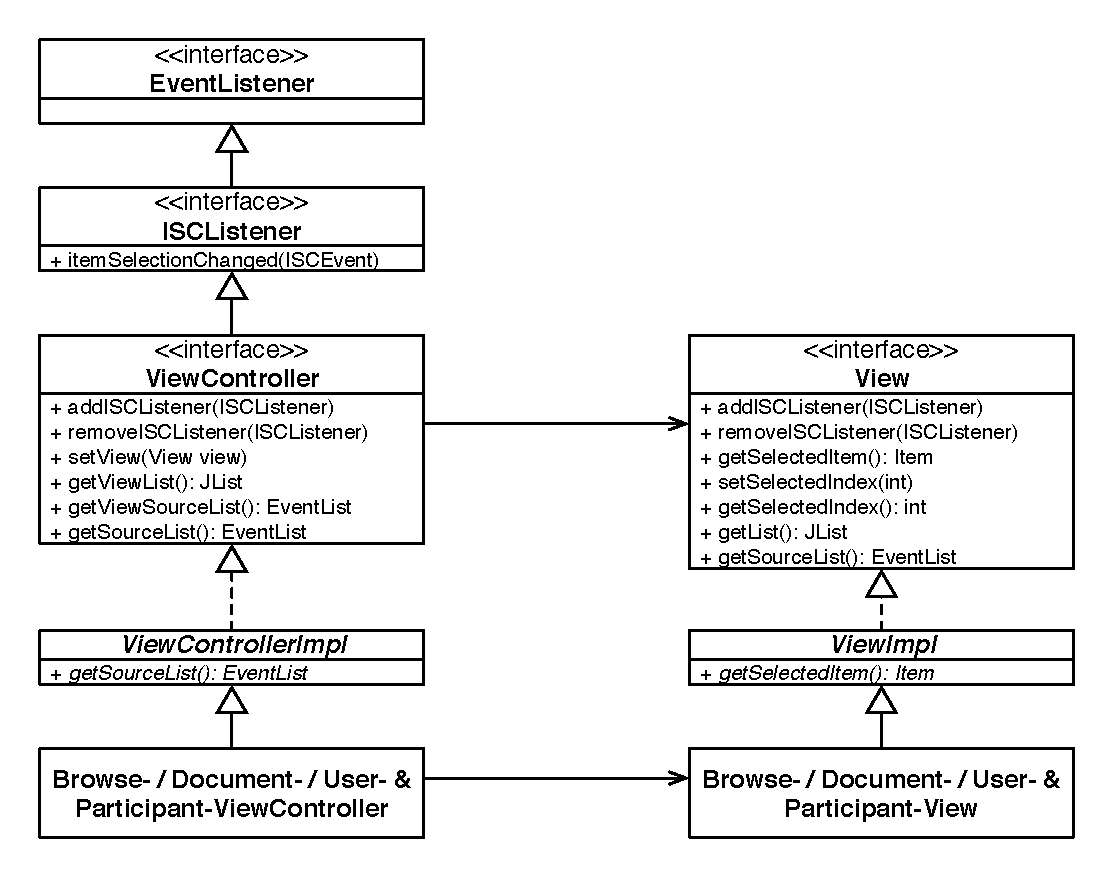
\includegraphics[height=5.62in, width=7.19in]{../images/finalreport/application_views_controllers.eps}
\caption{View \& ViewController Class Diagram}
\label{application_views_controllers}
\end{center}
\end{figure}

Each view has its own controller (e.g. a \texttt{Browse\-View} has a \texttt{Browse\-View\-Controller}). \texttt{View\-Controllers} are managing the data source of the \texttt{Views} and are needed to insert, remove or replace elements. The \texttt{View} itself displays only the elements of the data source. Moreover, a \texttt{View} returns the currently selected element to the \texttt{View\-Controller}. The construction of a \emph{View}/\emph{ViewController} pair consists of the following steps:

\begin{enumerate}
\item create the \texttt{View\-Controller}
\item create the \texttt{View} (code fragment from the contructor of \texttt{ViewImpl}):

  \begin{verbatim}
    public ViewImpl(ViewController controller, ...) {
      controller.setView(this);
      addItemSelectionChangeListener(controller);
    }
  \end{verbatim}
  
After the \texttt{View} has been created, it registers itself with the given \texttt{View\-Controller} (\texttt{controller.setView(this)}) and registers the controller as an \emph{Item\-Selection\-Change\-Listener} on the recipient list. The \emph{Item\-Selection\-Change\-Event}s are sent whenever the selection of the \texttt{View} has changed.
\end{enumerate}

% TODO: revise the following section
To keep the displayed list elements up to date \emph{Glazed Lists} are used. \emph{Glazed Lists} providing \texttt{Event\-Lists} which are observing their elements. If such an element changes a property (and fires a \texttt{firePropertyChange(...)}) the list will automatically be updated (see section \ref{appendix_frameworks_glazedlists} for more details).

The next four sections explain the usage of the four different \texttt{Views}.

\subsubsection{Document View \& Controller}
The \texttt{Document\-View} is used to display the currently open documents. An open document can either be a local document (new or an existing document on the local machine), a published document (a local document that has been published) or a joined document published by another user. All needed information for documents are contained in \texttt{Document\-Items}. The most important attributes are:

\begin{itemize}
\item Type: the type decides what kind of document the \texttt{Document\-Item} is needed for. Possible document types are: \emph{local} (private documents), \emph{published} (private documents that have been published), \emph{joined} (documents from other users that have been joined), \emph{remote} (documents from other users that have been discovered) and \emph{awaiting} (remote documents the joining process is running).
\item Editor Document: the styled document (see section \ref{applicationlayer_collabdocument}) that contains the content and is displayed in the text component.
\item If the type is \emph{remote} or \emph{published}: the \texttt{Session} and \texttt{Session\-Callback} are set to send and receive \texttt{Operations}.
\end{itemize}

\begin{figure}[H]
\begin{center}
  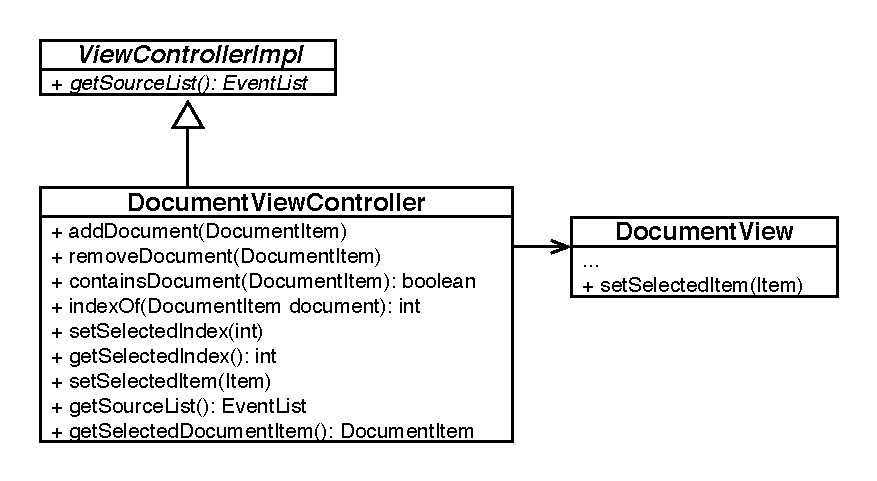
\includegraphics[height=2.99in, width=5.62in]{../images/finalreport/application_documentview.eps}
\caption{Document View Controller}
\label{application_documentview}
\end{center}
\end{figure}

The \texttt{DocumentItem} class is used for other document types than \emph{local}, \emph{published} or \emph{joined} too. To display only the local, published and joined documents, a so called \texttt{FilterList} is needed (see figure \ref{application_list_usage}).

\begin{figure}[H]
\begin{center}
  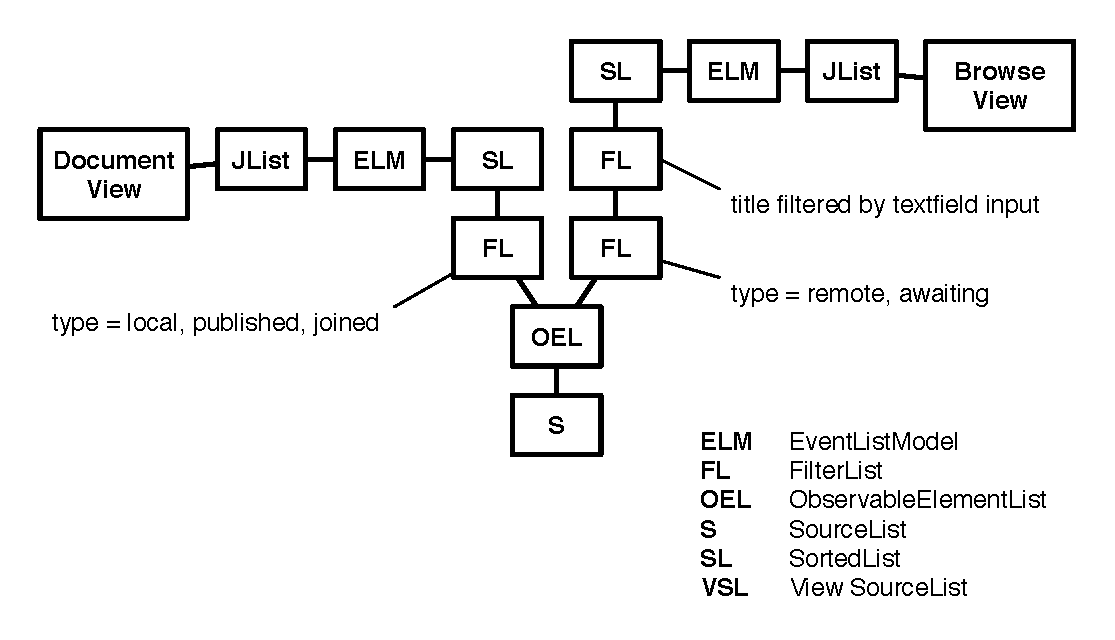
\includegraphics[height=3.24in, width=5.77in]{../images/finalreport/application_listusage.eps}
\caption{List construction used by Document- \& Browse-View}
\end{center}
\label{application_list_usage}
\end{figure} 

%\begin{verbatim}
%  Matcher documentViewMatcher = new Matcher() {
%    public boolean matches(Object item) {
%      DocumentItem dItem = (DocumentItem)item;
%      return (dItem.getType() == DocumentItem.LOCAL ||
%      dItem.getType() == DocumentItem.PUBLISHED ||
%      dItem.getType() == DocumentItem.JOINED);
%    }
%  };
%\end{verbatim}

\subsubsection{Browse View \& Controller}
The \texttt{Browse\-View} displays all documents published by other users that have been discovered. The \texttt{Browse\-View\-Controller}, which controls the \texttt{Browse\-View}, implements the \texttt{Document\-Listener} interface and is registered on the \texttt{Collaboration\-Service}. Whenever the controller is notified about document discovery events, it updates the source list of the view.

\begin{figure}[H]
\begin{center}
  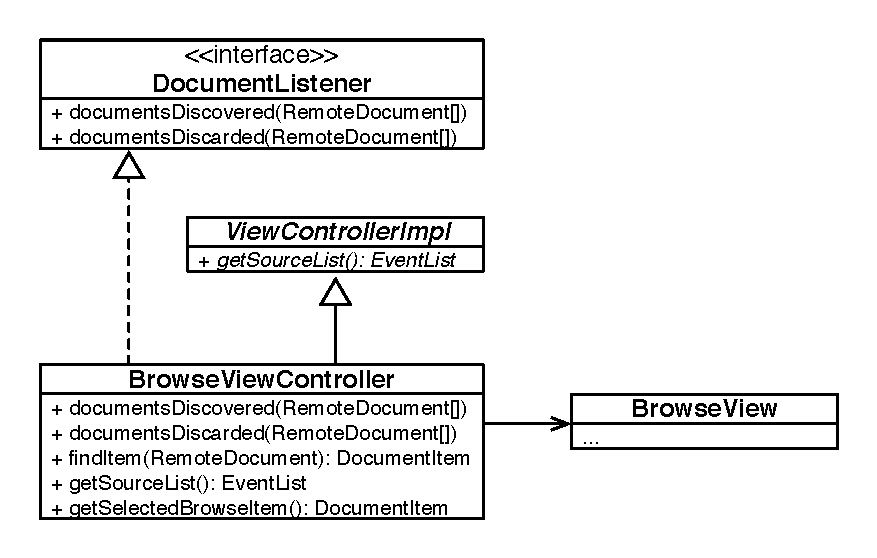
\includegraphics[height=3.5in, width=5.62in]{../images/finalreport/application_browseview.eps}
\caption{Browse View Controller}
\label{application_browseview}
\end{center}
\end{figure}

Because the \texttt{Browse\-View} uses the same source list of \texttt{Document\-Item} as the \texttt{Document\-View}, another filter (matcher) is needed to filter the documents based on their types. The \texttt{Browse\-View} only displays documents of type \emph{remote} and \emph{awaiting}. A \texttt{Document\-Item} has the type \emph{awaiting} while awaiting the response from the publisher to a join request.

% TODO: do not talk about matchers, filter lists...
%\begin{verbatim}
%  Matcher browseViewMatcher = new Matcher() {
%    public boolean matches(Object item) {
%      DocumentItem dItem = (DocumentItem)item;
%      return (dItem.getType() == DocumentItem.REMOTE ||
%      dItem.getType() == DocumentItem.AWAITING);
%    }
%  };
%\end{verbatim}

In case that there are a lot of users with a lot of published documents the \texttt{Browse\-View} has a filter included. This filter allows the user to type a publisher name into a text field. All documents that are not from this publisher will be filtered out and therefore not displayed.

%\begin{verbatim}
%  JTextField browseFilterField = new JTextField();
%  TextFilterator browseFilterator = new TextFilterator() {
%    public void getFilterStrings(List baseList, Object element) {
%      DocumentItem item = (DocumentItem)element;
%      baseList.add(item.getPublisher());
%    }
%  };
%\end{verbatim}

\subsubsection{User View \& Controller}
The \texttt{User\-View} displays all discovered users running ACE. The \texttt{User\-View\-Controller} implements the \texttt{User\-Listener} interface and is registered on the \texttt{Collaboration\-Service}. It receives a notification whenever a new user has been discovered or discarded from the network. It updates the source list accordingly. 

\begin{figure}[H]
\begin{center}
  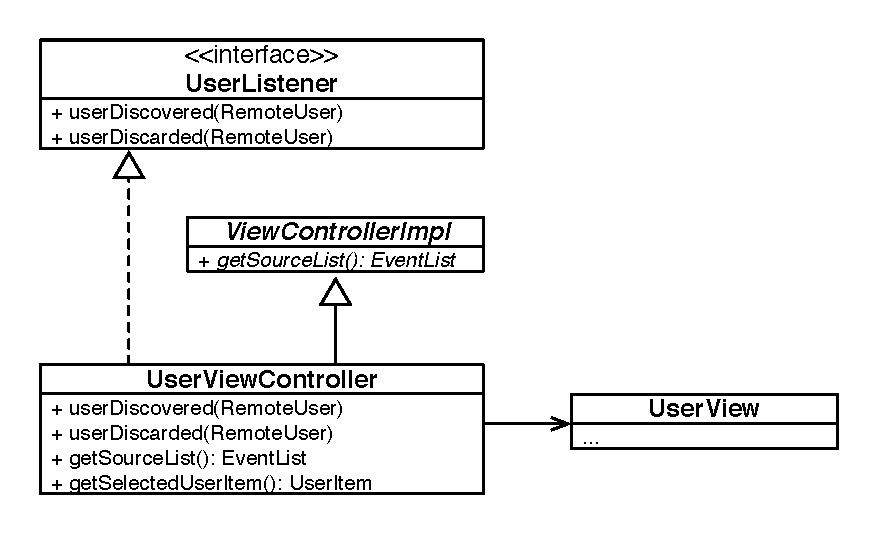
\includegraphics[height=3.33in, width=5.62in]{../images/finalreport/application_userview.eps}
\caption{User View Controller}
\label{application_userview}
\end{center}
\end{figure}

To find a user quickly from among all users, the \texttt{User\-View} has a filter. The filter is based on the text entered into a text field and compares that to the user names. All users not matching the entered text will be filtered out and are not displayed.

% TODO: what is a TextFilterator...
%\begin{verbatim}
%  JTextField userFilterField = new JTextField();
%  TextFilterator userFilterator = new TextFilterator() {
%    public void getFilterStrings(List baseList, Object element) {
%      UserItem item = (UserItem)element;
%      baseList.add(item.getName());
%    }
%  };
%\end{verbatim}

\subsubsection{Participant View \& Controller}
When a document is published a list of participants is created. At the beginning only the publisher of the document is in this list. For each user joining the document, a new \texttt{Participant\-Item} is created and added to the source list. The \texttt{Participant\-Item} contains the name of the participant and the color needed to highlight his text. The \texttt{Participant\-View} displays all \texttt{Participant\-Items} of the currently selected document.

\begin{figure}[H]
\begin{center}
  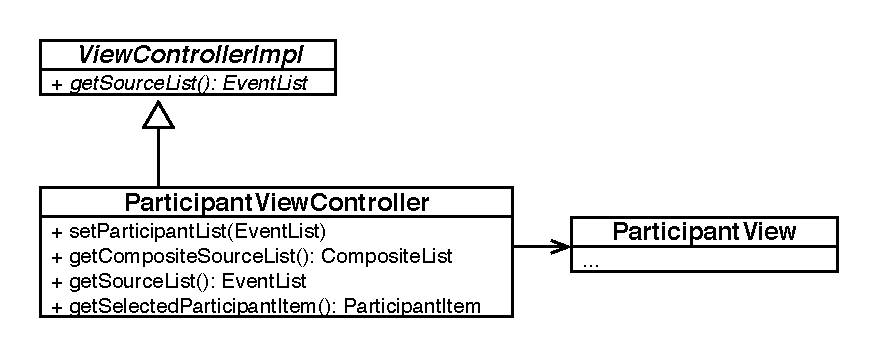
\includegraphics[height=2.15in, width=5.62in]{../images/finalreport/application_participantview.eps}
\caption{Participant View Controller}
\label{application_participantview}
\end{center}
\end{figure}

The \texttt{Session\-Callback} receives notifications from the collaboration layer about every participant joining or leaving the session updates the source list accordingly.

Each published document has its own list of participants which needs to be set in the \texttt{Participant\-View\-Controller} when the currently selected document changes.

% TODO: composite lists...

%\begin{verbatim}
%  public void setParticipantList(EventList participantList) {
%    // remove old participant list if there is one
%    if (memberList != null) {
%      participantSourceList.removeMemberList(memberList);
%    }
%
%    // add new participant list    
%    this.memberList = participantList;
%    participantSourceList.addMemberList(participantList);
%  }
%\end{verbatim}

% ACTIONS
\subsection{Actions}
All actions used by the application layer are subclasses of the \texttt{Abstract\-Action} class (which is part of \emph{Java Swing}). Actions have a \emph{name}, an \emph{icon} and optionally a \emph{shortcut} and a \emph{tooltip}. The \emph{name} and the \emph{icon} can be forwarded to the superclass. The following code fragment shows how to set the \emph{shortcut} and the \emph{tooltip}:

\begin{verbatim}
  // somewhere in costructor (shortcut = CTRL + X)
  putValue(ACCELERATOR_KEY, KeyStroke.getKeyStroke('X',
    Toolkit.getDefaultToolkit().getMenuShortcutKeyMask()));

  putValue(SHORT_DESCRIPTION, "Tooltip text here...");
\end{verbatim}

The behaviour of most of the actions depends on the current selection of the \texttt{Document\-View}. This leads to the \texttt{Document\-Item\-Selection\-Change\-Action} class:

\begin{figure}[H]
\begin{center}
  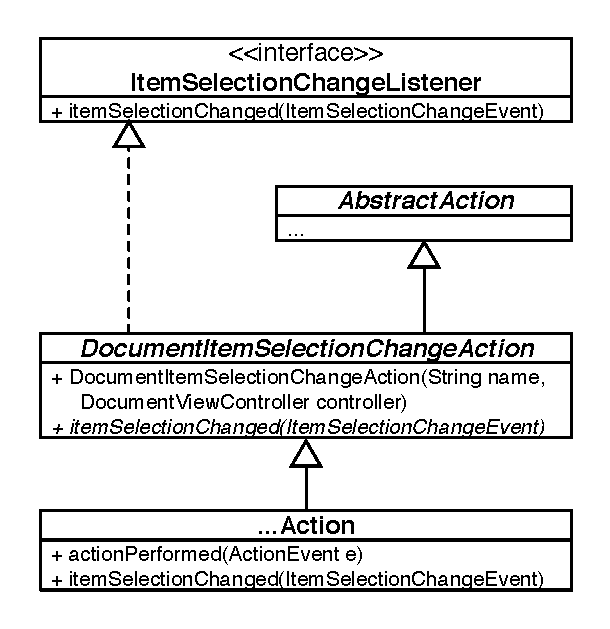
\includegraphics[height=3.97in, width=3.85in]{../images/finalreport/application_action.eps}
\caption{DocumentItemSelectionChangeAction Class Diagramm}
\label{application_application_action}
\end{center}
\end{figure}

This class handles the registration of the action to the \texttt{Item\-Selection\-Change\-Listener} of  the \texttt{Document\-View\-Controller}.

\begin{verbatim}
  public abstract class DocumentItemSelectionChangeAction
    extends AbstractAction implements ItemSelectionChangeListener {
  
    public DocumentItemSelectionChangeAction(String name, Icon icon,
          DocumentViewController viewController) {
      super(name, icon);
      viewController.addItemSelectionChangeListener(this);
    }
    
    public abstract void itemSelectionChanged(ItemSelectionChangeEvent e);
  }
\end{verbatim}

% ACTION ENABLING
It is important for the user-friendliness to enable or disable actions in the GUI. The enabling of most of the actions depends on the selection of the \texttt{Views}. For this pupose actions can register themselves on the view to receive \texttt{Item\-Selection\-Change\-Events}. Whenever the selection on the \texttt{View} changes, the method \texttt{itemSelectionChanged(...)} from the action is called.

For example the \emph{close document} action should only be enabled if a document is selected in the \texttt{Document\-View}:

\begin{verbatim}
  // somewhere in the constructor
  documentView.addItemSelectionChangeListener(this);

  public void itemSelectionChanged(ItemSelectionChangeEvent e) {
    if(e.getItem() == null) {
      // no document is selected
      setEnabled(false);
    } else {
      // a document is selected
      setEnabled(true);
    }
  }
\end{verbatim}

\newpage
% EDITOR
\subsection{Editor}
This section gives an overview of all components needed for the \texttt{Collaborative\-Editor}. The following figure shows the class diagram:
\begin{figure}[H]
\begin{center}
  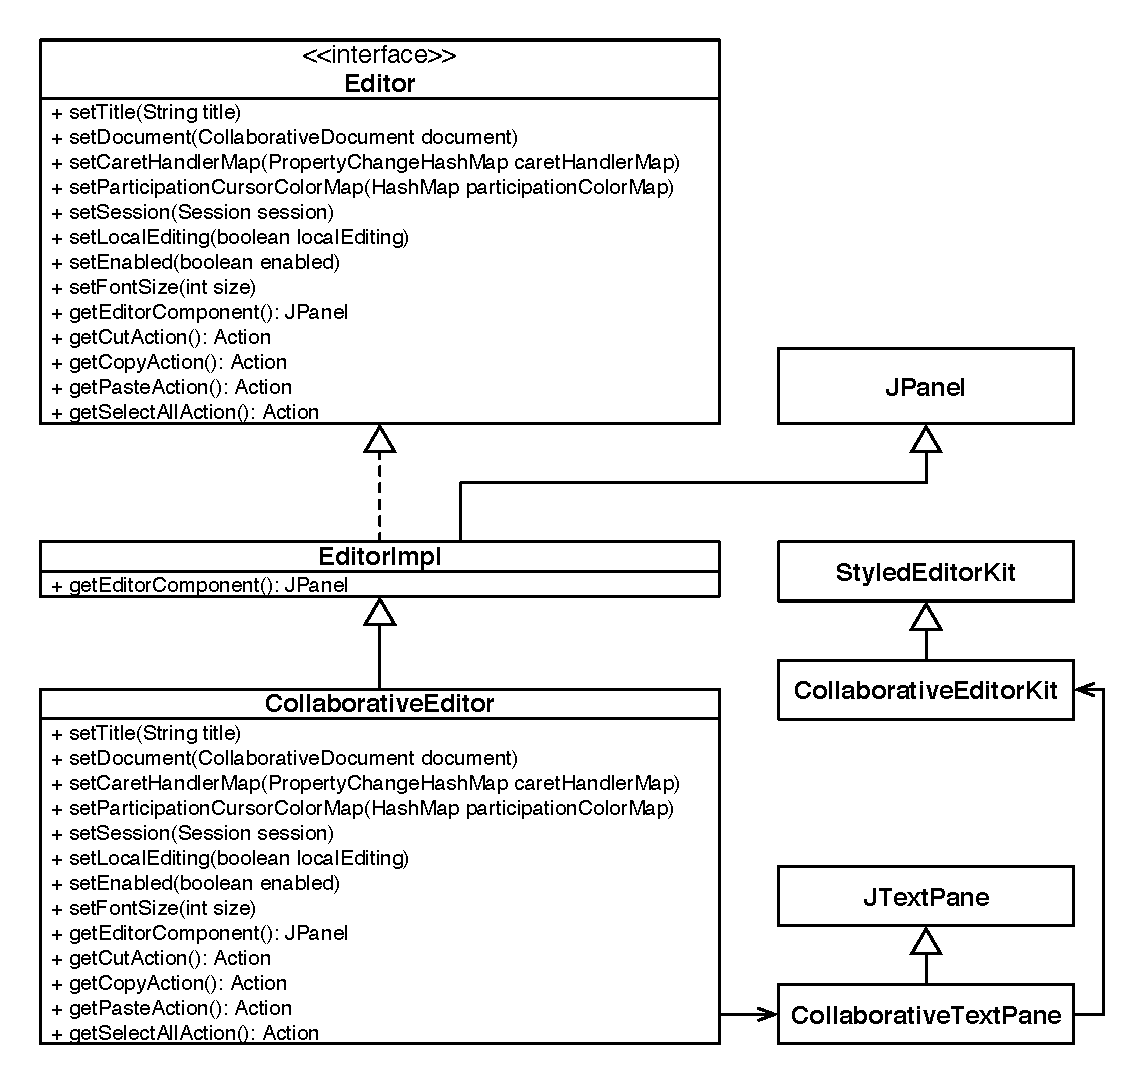
\includegraphics[height=5.25in, width=5.55in]{../images/finalreport/application_editor.eps}
\caption{Collaborative Editor Class Diagram}
\label{application_editor}
\end{center}
\end{figure}

\subsubsection{Collaborative Editor}
The \texttt{Collaborative\-Editor} is a \texttt{JPanel} which supports all the functionality defined in the \texttt{Editor} interface. The constructor looks like:
\begin{verbatim}
  public CollaborativeEditor(...) {
    // create editor pane & kit
    cTextPane = new CollaborativeTextPane();
    cEditorKit = new CollaborativeEditorKit();
    cTextPane.setEditorKit(cEditorKit);

    // create editor pane
    JScrollPane scrollPane = new JScrollPane(cTextPane);
    editorPane = new SimpleInternalFrame(null, " ", editorToolBar, scrollPane);

    // add components		
    setLayout(new BorderLayout());
    add(editorPane);    
  }
\end{verbatim}

All setter methods (except \texttt{setTitle(...)} that directly sets the title of the panel) are forwarded to the \texttt{Collaborative\-Text\-Pane} (\texttt{cTextPane}) like.

To use the standard \emph{Java Swing} text component actions in the \emph{Edit Menu}, getter methods are needed to return them. All these text component actions are handled in the \texttt{Editor\-Kit} (see section \ref{collaborative_editor_kit}), thus the getter methods are simply forwarded to the \texttt{Collaborative\-Editor\-Kit} (\texttt{cEditorKit}).


\subsubsection{Collaborative TextPane}
The \texttt{Collaborative\-Text\-Pane} subclasses the \texttt{JTextPane}. It overrides the \texttt{replaceSelection} method from its superclass. This is needed to include a lock while inserting text into the document. Locking has to be done to avoid asynchronous text insertions while creating and sending operations that are based on the document content.

\begin{verbatim}
  public void replaceSelection(String content) {
    SessionTemplate template = new SessionTemplate(session);
    template.execute(new SessionTemplateCallback() {
      public void execute(Session session) {

        // create and send operation
        Operation op  = new Delete/InsertOperation(...);
        session.sendOperation(op);

        // call superclass method
        CollaborativeTextPane.super.replaceSelection(content);
      }
    }
  }
\end{verbatim}

Furthermore, there is a method \texttt{setCaretHandlerMap(PropertyChangeHashMap caretHandlerMap)} which sets the map with the carets (cursor positions) from all participants of the current document. The \texttt{PropertyChangeHashMap} is a map that registers a \texttt{PropertyChangeListener} on all inserted elements (carets from other users) and forwards their \texttt{PropertyChangeEvents} to all registered components. The following code fragment makes the editor able to receive updates if the carets of other users have changed:

\begin{verbatim}
  public void setCaretHandlerMap(PropertyChangeHashMap caretHandlerMap) {
    // unregister old map
    this.caretHandlerMap.removePropertyChangeListener(this);
    this.caretHandlerMap = caretHandlerMap;

    // register new map
    this.caretHandlerMap.addPropertyChangeListener(this);
  }
\end{verbatim}

To handle the changes of the local caret it is necessary to register a \texttt{CaretListener}. The invoked method \texttt{caretUpdate(...)} checks if the cursor position has changed and sends the new caret position to the session.

Each time a caret of another user changes the method \texttt{propertyChange(PropertyChangeEvent evt)} will be invoked from the \texttt{Property\-Change\-Hash\-Map}. The \texttt{Property\-Change\-Event} contains the old and the new caret position from the user that moved his caret. A repaint of the old and the new cursor is needed. The implementation looks like:

\begin{verbatim}
  public void propertyChange(PropertyChangeEvent evt) {
    // old caret
    CaretUpdate oldCU = (CaretUpdate)evt.getOldValue();
    Rectangle oldRect = modelToView(oldCU.getDot());
    repaint(oldRect);

    // new caret
    CaretUpdate newCU = (CaretUpdate)evt.getNewValue();
    Rectangle newRect = modelToView(newCU.getDot());
    repaint(newRect);
  }
\end{verbatim}

The \texttt{repaint(...)} is either called by Swing or explicitly by the \texttt{propertyChange} method when one of the participants changed his cursor position. It iterates through the \texttt{caretHandlerMap} and paints the cursor of each user.

\subsubsection{Collaborative EditoKit}
\label{collaborative_editor_kit}
The \texttt{Collaborative\-Editor\-Kit} extends the \texttt{Styled\-Editor\-Kit} and is needed for synchronization purposes. To ensure the correct content of the text component it is necessary to lock the session before sending operation to the sesion in the following situations:

\begin{itemize}
\item \texttt{DeletePrevCharAction} which is called when the users presses the backspace key.
\item \texttt{DeleteNextCharAction} which is called when the users presses the delete key.
\item \texttt{CutAction} which is called when the user cuts some text out of the document.
\item Inserting Content: this issue is handled in the \texttt{Collaborative\-Text\-Pane}.
\end{itemize}

All editor actions are defined in an array that can be retrieved with the \texttt{getActions()} method from the superclass \texttt{StyledEditorKit}. The three delete actions listed above need to be replaced by actions that are able to use locks. A simple solution would be to subclass the action classes,
for instance \texttt{Default\-Editor\-Kit.Delete\-Prev\-Char\-Action}.

Unfortunately it is not possible to subclass the actions defined in the \texttt{DefaultEditorKit} because they are all package private. This leads to the solution to copy the implementations into the \texttt{Collaborative\-Editor\-Kit} class and manipulate them. For example the \texttt{actionPerformed} method of \texttt{DeletePrevCharAction} looks like:

\begin{verbatim}
  public void actionPerformed(...) {
    SessionTemplate template = new SessionTemplate(session);
    template.execute(new SessionTemplateCallback() {
      public void execute(Session session) {

        // check whatever needed here and manipulate text component document
        document.remove(...);
        
        // create and send operation
        Operation op  = new DeleteOperation(...);
        session.sendOperation(op);

      }
    }
  }
\end{verbatim}

The \texttt{Session\-Template} ensures proper locking/unlocking of the session. The actual user code is passed as an implementation of the \texttt{Session\-Template\-Callback} interface.


\subsubsection{Editor Controller}
The \texttt{Editor\-Controller} is registered for \texttt{Item\-Selection\-Change\-Events} from the \texttt{Document\-View\-Controller} and is used to enable, disable and set editor values. Each time the selection of the \texttt{Document\-View} or a property of the currently selected \texttt{Document\-Item} changes, the following steps are performed:

\begin{itemize}
\item \emph{disable} the editor if no document is selected. otherwise:
\item \emph{set} the \emph{document} of the selected item.
\item \emph{set} the editor \emph{title}.
\end{itemize}

If the selected document is a published or a joined (remote) document the \texttt{Session} is set too and the \emph{participant list} is updated in the \texttt{Participant\-View\-Controller}.

\subsubsection{Collaborative Document}
\label{applicationlayer_collabdocument}

The \texttt{Collaborative\-Document} extends the \texttt{Default\-Styled\-Document}. It is used for applying text styles. Each time a style added to the document changes the method \texttt{reapplyStyles(...)} is called. For each
participant there is a style that contains his background color.

\begin{verbatim}
  protected void styleChanged(Style style) {
    if(!style.getName().equals("default")) {
      reapplyStyles(style);
    }
  }
\end{verbatim}

Further, the \texttt{Collaborative\-Document} exposes the write lock of
the \texttt{Abstract\-Document}. This write lock is passed to the
collaboration layer from the \texttt{Session\-Callback}'s \texttt{get\-Lock}
method.

The method \texttt{reapplyStyles(...)} iterates through all the text elements of the document and checks if they are using the changed style. All elements using this style will be updated. \texttt{reapplyStyles} is used to update the text color when a participant leaves or rejoins the session. 

The following scenario will change the background color of all elements using the style "myStyle" from blue to red:
\begin{verbatim}
  // add style
  Style myStyle = document.addStyle("myStyle", null);
  StyleConstants.setBackground(myStyle, Color.BLUE);
  
  // insert some text here
  doc.insertString(...);
  
  // change style
  StyleConstants.setBackground(myStyle, Color.RED);
\end{verbatim}


\subsubsection{AsyncCaret}
When inserting text into a text component and setting the caret position asynchronously (from another thread than the AWT thread), the caret position is not updated. Asynchronous caret updates are implemented in Java 1.4 but there is no posibility to enable the feature (this problem is solved in Java 1.5). \texttt{Async\-Caret} is a simple copy of the standard caret class used by Swing which enables updating the caret position in case of asynchronous updates to the document

% OTHER
\subsection{Miscellaneous Information}
% APPLICATION FACTORY
\subsubsection{Application Factory}
\label{applicationlayer_applicationfactory}
To build the GUI (see section \ref{applicationlayer_wf_startup}) the \texttt{Application\-Factory} is used. It provides methods to create the \emph{Menu Bar}, the \emph{Tool Bar}, the \texttt{Persistent\-Component\-Pane} and the \emph{Status Bar}. Further, some parts of the GUI are created and wired by \emph{Spring} (see section \ref{appendix_frameworks_spring}). 

% DECIDE: remove following verbatim environment?
%\begin{verbatim}
%  public JMenuBar createMenuBar() {
%    JMenuBar menuBar = new JMenuBar();

%    JMenu m1 = new JMenu("Menu 1");
%    m1.add(...);        // add actions for menu 1
%    menuBar.add(m1);    // add menu 1 to the menubar
%    
%    JMenu m2 = new JMenu("Menu 2");
%    m2.add(...);        // add actions for menu 2
%    menuBar.add(m2);    // add menu 2 to the menubar
%    
%    return menuBar;
%  }
%\end{verbatim}

% DECIDE: remove following verbatim environment?
%\begin{verbatim}
%  public JToolBar createToolBar() {
%    JToolBar toolBar = new JToolBar();
%    toolBar.setFloatable(false);   // make it impossible to drag the toolbar
%    toolBar.setRollover(true);

%    toolBar.add(...);   // add actions to toolbar

%    return toolBar;
%  }
%\end{verbatim}


% APPLICATION CONTROLLER
\subsubsection{Application Controller}
All functions that may need to show a dialog for user input or for displaying errors are handled within the \texttt{Application\-Controller}. Some functions like for example \texttt{closeDocument()} need to do some checks before they open a dialog and other functions like \texttt{showAbout()} directly pop up the required dialog. To show dialogs the \texttt{Application Controller} uses the \texttt{Dialog\-Controller} (\ref{applicationlayer_dialogcontroller}).

% DIALOG CONTROLLER
\subsubsection{Dialog Controller}
\label{applicationlayer_dialogcontroller}
The \texttt{Dialog\-Controller} is used to display dialogs. These dialogs are either used to get user input or to notify the user. 

By separating the code that displays dialogs from the logic that decides when
to show a dialog it was possible to thoroughly unit test the \texttt{Application\-Controller}. The \texttt{Dialog\-Controller} interface can be mocked and thus the possible decisions made by the user can be tested quite easily.



% PERSISTENT CONTENT PANE
\subsubsection{Persistent Content Pane}
The \texttt{Persistent\-Content\-Pane} is the container for all \texttt{Views} and the \texttt{Editor} component. It is a \texttt{JPanel} containing several \emph{split panes} to make the GUI components resizable (see figure \ref{application_splitpane}).

\begin{figure}[H]
\begin{center}
  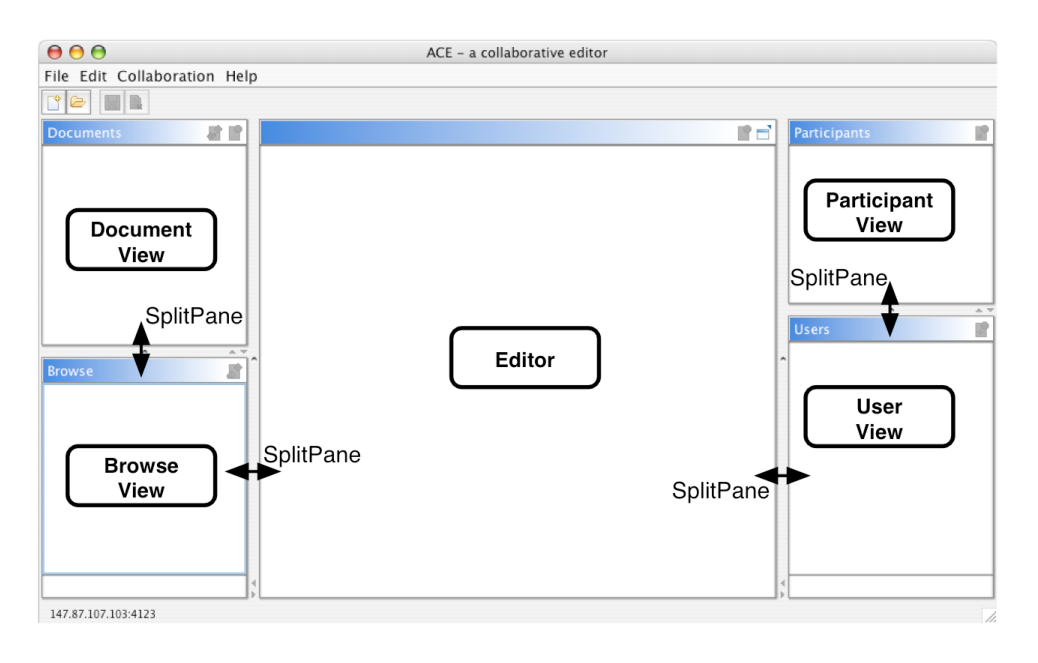
\includegraphics[height=4.19in, width=6.69in]{../images/finalreport/application_splitpane.eps}
\caption{Persistent SplitPane}
\label{application_splitpane}
\end{center}
\end{figure}

% TODO: see User Manual section x.y.z
The special method \texttt{switchFullScreenEditing()} maximizes the \texttt{Editor} and minimizes all other components. For the usage of this feature see \emph{User Manual, section 3.3: Editor}.



% WORKFLOWS
\section{Workflows}

% STARTUP
\subsection{Startup}
\label{applicationlayer_wf_startup}
The startup process of ACE is defined in the main method of the class \texttt{Main}. It consists of the following steps:
\begin{description}
\item[1. Load Customizer ] The first step is to get the customizers. Customizers are used to create operating system based stuff like setting the look \& feel of the application. Customizers also support handling OS X specific events, like for instance opening a file when the user is dropping a file onto the application icon.
\item[2. Load ApplicationContext ] After the customizer has been loaded, the Spring application context (see \ref{appendix_frameworks_spring} for more details about spring) is loaded. With the help of the \texttt{Application\-Context} the \texttt{Application\-Factory}, the \texttt{Application\-Controller} and the \texttt{Collaboration\-Service} are created and initialized.
\item[3. Create Main Frame ] With the help of the \texttt{Application\-Factory} the \emph{Menu}, \emph{Toolbar} and the \emph{Content Pane} (which includes all \emph{Views} and the \emph{Editor}) are loaded and integrated into the GUI.
\item[4. Load Preferences Store ] The \texttt{Preferences\-Store} needs to be loaded to get the unique user id which is needed to initialize the \texttt{Collaboration\-Service}.
\item[5. Init Collaboration Service ] The \texttt{Collaboration\-Service} needs to be initialized. This includes setting the local user details, the \texttt{Invitation\-Callback} and \texttt{Service\-Failure\-Handler}. After all necessary properties are set, the \texttt{Collaboration\-Service} can be started.
\item[6. Create Empty Document ] ACE opens an empty document, which makes it possible for the user to immediately start writing once the application is started.
\end{description}

